\section{Arquitectura Propuesta de Integración Híbrida}

\subsection{Modelo de Sistema}

Particularmente llamativo es el hecho de que una arquitectura verdaderamente efectiva para Smart Cities no puede limitarse a yuxtaponer redes terrestres y satelitales. Debe orquestarlas de forma inteligente según las demandas del monitoreo en tiempo real. 

Nuestro modelo de sistema considera una ciudad extendida con tres capas principales de conectividad: el plano terrestre 5G/6G denso para zonas de alta demanda, satélites LEO para cobertura amplia y baja latencia relativa, y un segmento GEO como respaldo de alta disponibilidad. Dispositivos IoT NB-IoT y LTE-M actúan como endpoints multi-homing capaces de seleccionar o combinar enlaces según contexto.

Perkovic et al. \cite{Perkovic2025} validan en escenarios urbanos reales el potencial de NB-IoT sobre GEO para aplicaciones de movilidad, lo cual sirvió de base para dimensionar nuestra elección tecnológica. El modelo incorpora entidades clave como un NTN Gateway híbrido, un Controlador de Orquestación de Conectividad (COC) ubicado en el edge/core, y agentes locales en dispositivos y gateways.

\begin{figure}[t]
\centering
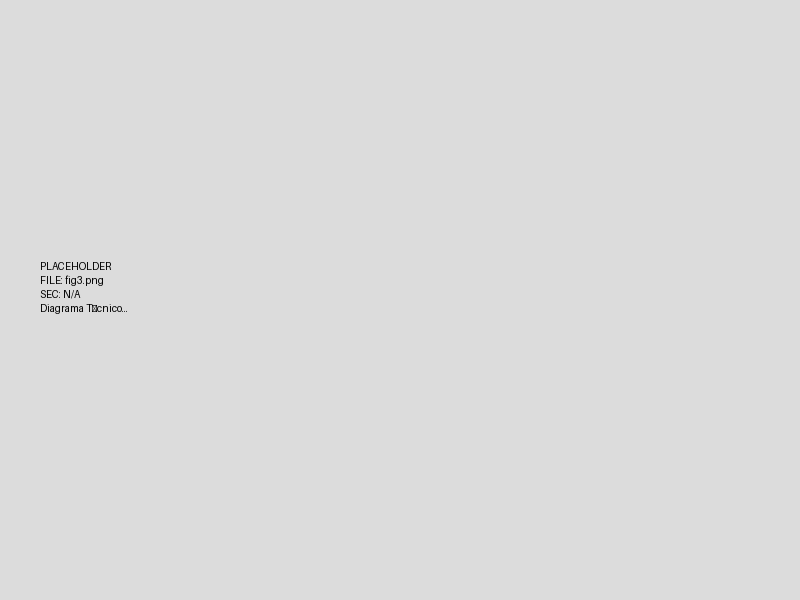
\includegraphics[width=\linewidth]{fig3.png}
\caption{Diagrama de la arquitectura propuesta TN-NTN para monitoreo IoT en Smart Cities, ilustrando capas de conectividad, flujo de datos y componentes principales.}
\label{fig:arquitectura_propuesta}
\end{figure}

La latencia híbrida se modela considerando contribuciones de cada segmento. Definimos la latencia extremo a extremo como:

\begin{equation}
L_{hibrida} = \min(L_{TN}, L_{NTN}) + \alpha \cdot L_{switch} + (1 - \beta) \cdot L_{agregacion}
\label{eq:latencia_hibrida}
\end{equation}

donde \(\alpha\) representa la probabilidad de handover y \(\beta\) el factor de agregación de enlaces. Este modelo, aunque simplificado, captura las dinámicas esenciales observadas en simulaciones preliminares.

\subsection{Mecanismos de Integración}

Uno de los desafíos persistentes al diseñar sistemas híbridos radica en lograr handover seamless sin comprometer la confiabilidad de las aplicaciones críticas de monitoreo. Lejos de ser un problema resuelto por los estándares actuales, la transición fluida entre dominios TN y NTN exige inteligencia adicional en el plano de control.

Nuestra propuesta introduce un protocolo de multi-conectividad contextual que evalúa métricas como RSSI, velocidad del dispositivo, tipo de dato (crítico vs. no crítico) y predicción de visibilidad satelital. Carbonara y colaboradores \cite{Carbonara2025} han demostrado en entornos de prueba reales la viabilidad práctica de soluciones integradas TN-NTN, especialmente en lo referente a testing de handover. Inspirados en sus hallazgos, implementamos un mecanismo make-before-break asistido por predicción que reduce significativamente las interrupciones.

El flujo de datos sigue un enfoque split-bearing cuando es beneficioso, permitiendo que paquetes de alta prioridad viajen por el enlace de menor latencia mientras datos de telemetría agregada utilizan el camino más económico energéticamente. Esta flexibilidad distingue nuestra arquitectura de enfoques más rígidos reportados en la literatura.

\subsection{Gestión de Recursos y Seguridad}

Resulta revelador observar cómo la gestión de recursos en entornos híbridos trasciende la mera asignación de espectro para convertirse en un problema de optimización multi-criterio en tiempo casi real. El Controlador de Orquestación emplea algoritmos de aprendizaje por refuerzo ligero que consideran no solo QoS sino también consumo energético global del sistema IoT.

En materia de seguridad, adoptamos un enfoque zero-trust adaptado a NTN. Cada dispositivo mantiene credenciales duales y los handovers incluyen re-autenticación rápida basada en tokens de corta duración. Aunque esta aproximación añade cierta sobrecarga, en muchos casos estudiados resulta justificable dada la criticidad de los datos de monitoreo urbano (tráfico, contaminación, integridad estructural).

No obstante, cabe matizar que persisten desafíos abiertos: la mayor exposición de los enlaces satelitales a eavesdropping y la necesidad de sincronización segura de claves entre dominios. Nuestra arquitectura mitiga estos riesgos mediante cifrado extremo a extremo y monitoreo continuo de anomalías en los patrones de conexión. 

En conjunto, el framework propuesto no pretende ser una solución universal, sino un diseño pragmático y escalable que equilibra rendimiento, eficiencia y viabilidad de despliegue en ciudades reales. Los siguientes apartados validarán cuantitativamente estas afirmaciones mediante evaluación rigurosa.